%package list
\documentclass{article}
\usepackage[top=3cm, bottom=3cm, outer=3cm, inner=3cm]{geometry}
\usepackage{multicol}
\usepackage{graphicx}
\usepackage{url}
%\usepackage{cite}
\usepackage{hyperref}
\usepackage{array}
%\usepackage{multicol}
\newcolumntype{x}[1]{>{\centering\arraybackslash\hspace{0pt}}p{#1}}
\usepackage{natbib}
\usepackage{pdfpages}
\usepackage{multirow}
\usepackage[normalem]{ulem}
\useunder{\uline}{\ul}{}
\usepackage{svg}
\usepackage{xcolor}
\usepackage{listings}
\lstdefinestyle{ascii-tree}{
    literate={├}{|}1 {─}{--}1 {└}{+}1 
  }
\lstset{basicstyle=\ttfamily,
  showstringspaces=false,
  commentstyle=\color{red},
  keywordstyle=\color{blue}
}
%\usepackage{booktabs}
\usepackage{caption}
\usepackage{subcaption}
\usepackage{float}
\usepackage{array}

\newcolumntype{M}[1]{>{\centering\arraybackslash}m{#1}}
\newcolumntype{N}{@{}m{0pt}@{}}


%%%%%%%%%%%%%%%%%%%%%%%%%%%%%%%%%%%%%%%%%%%%%%%%%%%%%%%%%%%%%%%%%%%%%%%%%%%%
%%%%%%%%%%%%%%%%%%%%%%%%%%%%%%%%%%%%%%%%%%%%%%%%%%%%%%%%%%%%%%%%%%%%%%%%%%%%
\newcommand{\itemEmail}{rvaldiviase@unsa.edu.pe}
\newcommand{\itemStudent}{Ryan Fabian Valdivia Segovia}
\newcommand{\itemCourse}{Fundamentos de la programación 2}
\newcommand{\itemCourseCode}{1701213}
\newcommand{\itemSemester}{II}
\newcommand{\itemUniversity}{Universidad Nacional de San Agustín de Arequipa}
\newcommand{\itemFaculty}{Facultad de Ingeniería de Producción y Servicios}
\newcommand{\itemDepartment}{Departamento Académico de Ingeniería de Sistemas e Informática}
\newcommand{\itemSchool}{Escuela Profesional de Ingeniería de Sistemas}
\newcommand{\itemAcademic}{2023 - B}
\newcommand{\itemInput}{Del 11 de Octubre 2023}
\newcommand{\itemOutput}{Al 16 de Octubre 2023}
\newcommand{\itemPracticeNumber}{05}
\newcommand{\itemTheme}{Arreglos bidimensionales de objetos}
%%%%%%%%%%%%%%%%%%%%%%%%%%%%%%%%%%%%%%%%%%%%%%%%%%%%%%%%%%%%%%%%%%%%%%%%%%%%
%%%%%%%%%%%%%%%%%%%%%%%%%%%%%%%%%%%%%%%%%%%%%%%%%%%%%%%%%%%%%%%%%%%%%%%%%%%%

\usepackage[english,spanish]{babel}
\usepackage[utf8]{inputenc}
\AtBeginDocument{\selectlanguage{spanish}}
\renewcommand{\figurename}{Figura}
\renewcommand{\refname}{Referencias}
\renewcommand{\tablename}{Tabla} %esto no funciona cuando se usa babel
\AtBeginDocument{%
	\renewcommand\tablename{Tabla}
}

\usepackage{fancyhdr}
\pagestyle{fancy}
\fancyhf{}
\setlength{\headheight}{30pt}
\renewcommand{\headrulewidth}{1pt}
\renewcommand{\footrulewidth}{1pt}
\fancyhead[L]{\raisebox{-0.2\height}{
\includegraphics[width=3cm]{img/logo_episunsa.png}}}
\fancyhead[C]{\fontsize{7}{7}\selectfont	\itemUniversity \\ \itemFaculty \\ \itemDepartment \\ \itemSchool \\ \textbf{\itemCourse}}
\fancyhead[R]{\raisebox{-0.2\height}{
\includegraphics[width=1.2cm]{img/logo_abet}}}
\fancyfoot[L]{Estudiante Ryan Valdivia}
\fancyfoot[C]{\itemCourse}
\fancyfoot[R]{Página \thepage}

% para el codigo fuente
\usepackage{listings}
\usepackage{color, colortbl}
\definecolor{dkgreen}{rgb}{0,0.6,0}
\definecolor{gray}{rgb}{0.5,0.5,0.5}
\definecolor{mauve}{rgb}{0.58,0,0.82}
\definecolor{codebackground}{rgb}{0.95, 0.95, 0.92}
\definecolor{tablebackground}{rgb}{0.8, 0, 0}

\lstset{frame=tb,
	language=bash,
	aboveskip=3mm,
	belowskip=3mm,
	showstringspaces=false,
	columns=flexible,
	basicstyle={\small\ttfamily},
	numbers=none,
	numberstyle=\tiny\color{gray},
	keywordstyle=\color{blue},
	commentstyle=\color{dkgreen},
	stringstyle=\color{mauve},
	breaklines=true,
	breakatwhitespace=true,
	tabsize=3,
	backgroundcolor= \color{codebackground},
}

\begin{document}
	
	\vspace*{10px}
	
	\begin{center}	
		\fontsize{17}{17} \textbf{ Informe de Laboratorio \itemPracticeNumber}
	\end{center}
	\centerline{\textbf{\Large Tema: \itemTheme}}
	%\vspace*{0.5cm}	

	\begin{flushright}
		\begin{tabular}{|M{2.5cm}|N|}
			\hline 
			\rowcolor{tablebackground}
			\color{white} \textbf{Nota}  \\
			\hline 
			     \\[30pt]
			\hline 			
		\end{tabular}
	\end{flushright}	

	\begin{table}[H]
		\begin{tabular}{|x{4.7cm}|x{4.8cm}|x{4.8cm}|}
			\hline 
			\rowcolor{tablebackground}
			\color{white} \textbf{Estudiante} & \color{white}\textbf{Escuela}  & \color{white}\textbf{Asignatura}   \\
			\hline 
			{\itemStudent \par \itemEmail} & \itemSchool & {\itemCourse \par Semestre: \itemSemester \par Código: \itemCourseCode}     \\
			\hline 			
		\end{tabular}
	\end{table}		
	
	\begin{table}[H]
		\begin{tabular}{|x{4.7cm}|x{4.8cm}|x{4.8cm}|}
			\hline 
			\rowcolor{tablebackground}
			\color{white}\textbf{Laboratorio} & \color{white}\textbf{Tema}  & \color{white}\textbf{Duración}   \\
			\hline 
			\itemPracticeNumber & \itemTheme & 04 horas   \\
			\hline 
		\end{tabular}
	\end{table}
	
	\begin{table}[H]
		\begin{tabular}{|x{4.7cm}|x{4.8cm}|x{4.8cm}|}
			\hline 
			\rowcolor{tablebackground}
			\color{white}\textbf{Semestre académico} & \color{white}\textbf{Fecha de inicio}  & \color{white}\textbf{Fecha de entrega}   \\
			\hline 
			\itemAcademic & \itemInput &  \itemOutput  \\
			\hline 
		\end{tabular}
	\end{table}
	
	\section{Tarea}
	\begin{itemize}
		\subsection{Videojuego}
			\item Cree un Proyecto llamado Laboratorio5.
			\item Usted deberá crear las dos clases Soldado.java y VideoJuego2.java. Puede reutilizar lo
desarrollado en Laboratorio 3 y 4.
			\item Del Soldado nos importa el nombre, puntos de vida, fila y columna (posición en el tablero).
			\item El juego se desarrollará en el mismo tablero de los laboratorios anteriores. Pero ahora el
tablero debe ser un arreglo bidimensional de objetos.
			\item Inicializar el tablero con n soldados aleatorios entre 1 y 10. Cada soldado tendrá un nombre
autogenerado: Soldado0, Soldado1, etc., un valor de puntos de vida autogenerado
aleatoriamente [1..5], la fila y columna también autogenerados aleatoriamente (no puede
haber 2 soldados en el mismo cuadrado). Se debe mostrar el tablero con todos los soldados
creados. Además de los datos del Soldado con mayor vida,
el promedio de puntos de vida de todos los soldados creados, el nivel de vida de todo el
ejército, los datos de todos los soldados en el orden que fueron creados y un ranking de poder
de todos los soldados creados, del que tiene más nivel de vida al que tiene menos (usar al
menos 2 algoritmos de ordenamiento).
	\end{itemize}
		
	\section{Equipos, materiales y temas utilizados}
	\begin{itemize}
		\item Sistema Operativo Windows 11 Home Single Language 64 bits 22621.2283
		\item VIM 9.0.
		\item Visual Studio Code 64 bits 1.82.2
		\item OpenJDK 64-Bits 11.0.16.1
		\item Git 2.41.0.windows.1
		\item Cuenta en GitHub con el correo institucional. 
	\end{itemize}
	
	\section{URL de Repositorio Github}
	\begin{itemize}
		\item URL del Repositorio GitHub para clonar o recuperar.
		\item \url{https://github.com/RyanValdivia/fp2-23b.git}
		\item URL para el laboratorio 05 en el Repositorio GitHub.
		\item \url{https://github.com/RyanValdivia/fp2-23b/tree/main/fase02/lab05}
	\end{itemize}
	
	\section{Actividades}
	\subsection{Actividad 1}
	
	\begin{itemize}	
		\item En primer lugar, realicé un commit conteniendo el código de la clase Soldado.java, requerido para la actividad principal.
	\end{itemize}	
	\begin{lstlisting}[language=bash,caption={Comentando el código de Soldado.java}][H]
		$ git log lab05
		commit a802a60b50724d01c56a86864d25c31caae71ce1
		Author: RYAN VALDIVIA <rvaldiviase@unsa.edu.pe>
		Date:   Sun Oct 15 21:13:11 2023 -0500
			Creando la clase 'Soldado.java' y trabajando el codigo principal, inicializando el arreglo de objetos bidimensional
	\end{lstlisting}
	\begin{itemize}	
		\item Conteniendo el siguiente código
	\end{itemize}
	\begin{lstlisting}[language=java,caption={Clase Soldado}, numbers=left][H]
public class Soldado {
    private String nombre;
    private int vida;
    private int fila;
    private int columna;

    public void setNombre(String s) {
        this.nombre = s;
    }

    public void setVida(int n) {
        this.vida = n;
    }

    public void setFila(int n) {
        this.fila = n;
    }

    public void setColumna(int n) {
        this.columna = n;
    }

    public String getNombre() {
        return nombre;
    }

    public int getVida() {
        return vida;
    }

    public int getFila() {
        return fila;
    }

    public int getColumna() {
        return columna;
    }
}
	\end{lstlisting}
	\begin{itemize}	
		\item Seguidamente, comencé elaborando los métodos requeridos para el funcionamiento del videojuego, por lo tanto, según mi lógica, lo primero era desplegar a los soldados en localizaciones aleatorias, sin que dos soldados estén en la misma casilla.
		\item Para esto, se me ocurrio crear dos arreglos de numeros enteros con numeros aleatorios, para luego tomar pares ordenados y asi formar coordenadas para los soldados sin que se repitan.
	\end{itemize}
	\begin{lstlisting}[language=java,caption={Números aleatorios}, numbers=left][H]
	public static int[] numerosRandom(int q) {
        int[] nums = new int[q];
        for (int i = 0; i < nums.length; i++) {
            nums[i] = nums.length;
        }
        for (int i = 0; i < q; i++) {
            int n;
            do {
                n = (int) (Math.random() * 10);
            } while (estaEnArreglo(nums, n, i));
            nums[i] = n;
        }
        return nums;
    }
	\end{lstlisting}
	\begin{lstlisting}[language=java,caption={Comprobar que no se repitan}, numbers=left][H]
	public static boolean estaEnArreglo(int[] arreglo, int num, int indice) {
        for (int i = 0; i < indice; i++) {
            if (arreglo[i] == num) {
                return true;
            }
        }
        return false;
    }
	\end{lstlisting}
	\begin{itemize}	
		\item Una vez ya hecho el sistema para obtener las coordenadas, realicé un método para inicializar el arreglo bidimensional, dadas las coordenadas, así estableciendo todos sus respectivos atributos a todos los objetos.
	\end{itemize}
	\begin{lstlisting}[language=java,caption={Inicializando el ejército}, numbers=left][H]
	public static void inicializarArreglo(Soldado[][] army, int[] filas, int[] columnas) {
        for (int i = 0; i < filas.length; i++) {
            int v = (int) ((Math.random() * 5) + 1);
            army[filas[i]][columnas[i]] = new Soldado();
            army[filas[i]][columnas[i]].setNombre("Soldado" + i);
            army[filas[i]][columnas[i]].setVida(v);
            army[filas[i]][columnas[i]].setFila(filas[i]);
            army[filas[i]][columnas[i]].setColumna(columnas[i]);
        }
    }
	\end{lstlisting}
	\begin{itemize}	
		\item Una vez inicializado, en el siguiente commit, creé el método para mostrar todo el tablero, con separadores para que se vea ésteticamente adecuado.
	\end{itemize}
	\begin{lstlisting}[language=java,caption={Mostrar el tablero}, numbers=left][H]
	public static void mostrarTablero(Soldado[][] army) {
        String vacio = "        ";
        System.out.println(crearTecho());
        for (int i = 0; i < army.length; i++) {
            System.out.println(separadorSup());
            for (int j = 0; j < army.length; j++) {
                if (j == army.length - 1) {
                    if (army[i][j] == null) {
                        System.out.print("| " + vacio + " |");
                    } else {
                        System.out.print("| " + army[i][j].getNombre() + " |");
                    }
                } else {
                    if (army[i][j] == null) {
                        System.out.print("| " + vacio + " ");
                    } else {
                        System.out.print("| " + army[i][j].getNombre() + " ");
                    }
                }
            }
            System.out.println();
            System.out.println(separadorInf());
        }
    }
	\end{lstlisting}	
	\begin{itemize}	
		\item Para que esto se vea bonito de forma estética, creé varios métodos para poder armar el tablero.
	\end{itemize}
	\begin{lstlisting}[language=java,caption={Método para la fila superior del todo}, numbers=left][H]
	 public static String crearTecho() {
        String franky = "";
        for (int i = 0; i < 111; i++) {
            franky += "_";
        }
        return franky;
    }
	\end{lstlisting}
	\begin{lstlisting}[language=java,caption={Método para separar las lineas(Parte superior)}, numbers=left][H]
	 public static String separadorSup() {
        String franky = "";
        for (int i = 0; i < 111; i++) {
            if (i % 11 == 0) {
                System.out.print("|");
            } else {
                System.out.print(" ");
            }
        }
        return franky;
    }
	\end{lstlisting}
	\begin{lstlisting}[language=java,caption={Método para separar las lineas(Parte inferior)}, numbers=left][H]
	 public static String separadorInf() {
        String franky = "";
        for (int i = 0; i < 111; i++) {
            if (i % 11 == 0) {
                System.out.print("|");
            } else {
                System.out.print("_");
            }
        }
        return franky;
    }
	\end{lstlisting}
	
	\begin{itemize}
		\item Imprimiendo esto al momento de ejecutar el código.
	\end{itemize}
	
	\begin{figure}[H]
		\centering
	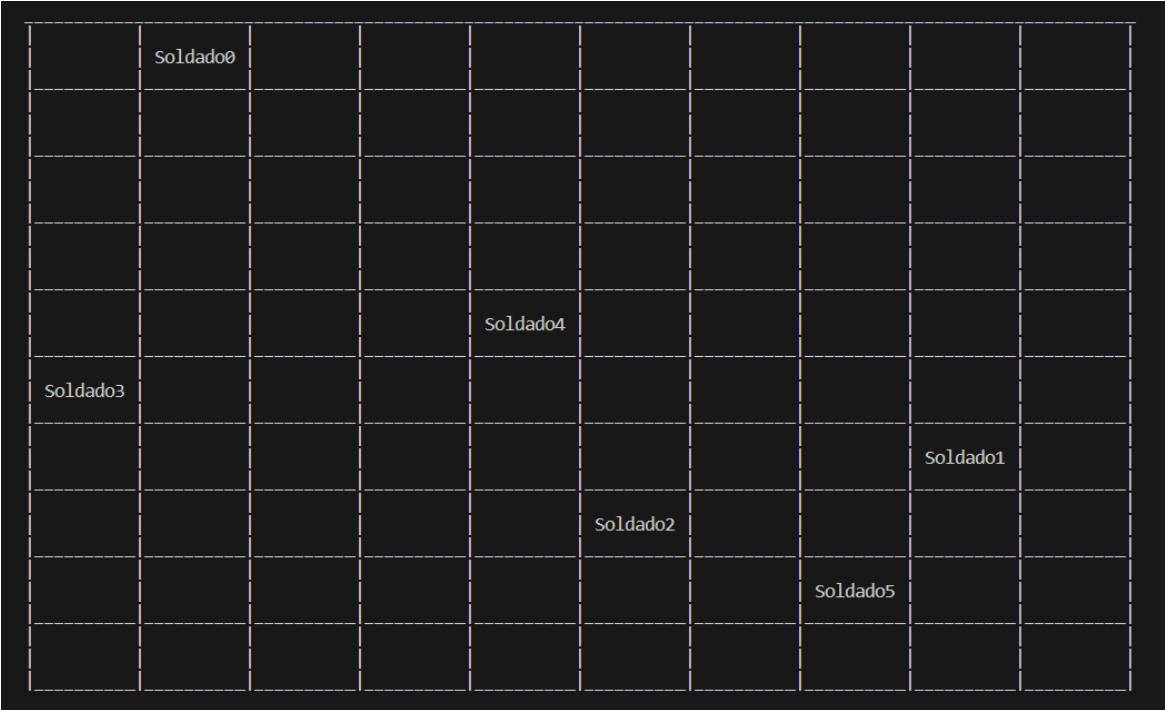
\includegraphics[width=0.8\textwidth,keepaspectratio]{img/captura1.png}
		%\includesvg{img/automata.svg}
		%\label{img:mot2}
		%\caption{Product backlog.}
	\end{figure}
	
	\begin{itemize}	
		\item Luego de esto, en el siguiente commit, trabajé el método para determinar el soldado con mayor vida del arreglo.
		\item Lo hice simplemente recorriendo todos los soldados y obteniendo los indices del soldado con mayor vida.
	\end{itemize}
	\begin{lstlisting}[language=java,caption={Soldado con mayor nivel de vida}, numbers=left][H]
	 public static void soldadoMayorVida(Soldado[][] army, int[] filas, int[] columnas) {
        int max = 0;
        for (int i = 0; i < filas.length; i++) {
            if (army[filas[i]][columnas[i]].getVida() > army[filas[max]][columnas[max]].getVida()) {
                max = i;
            }
        }
        System.out.println("El soldado con mayor vida es: ");
        mostrarSoldado(army, filas[max], columnas[max]);
    }
	\end{lstlisting}
	\begin{itemize}	
		\item Siguiendo con la ejecución de la anterior captura, nos imprimiría lo siguiente.
	\end{itemize}
	
	\begin{figure}[H]
		\centering
	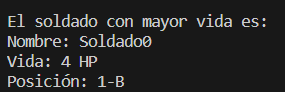
\includegraphics[width=0.4\textwidth,keepaspectratio]{img/captura2.png}
		%\includesvg{img/automata.svg}
		%\label{img:mot2}
		%\caption{Product backlog.}
	\end{figure}
	
	\begin{itemize}	
		\item Además, por motivos de conveniencia, decidí crear un método para mostrar todos los datos de un soldado en la consola, siéndome útil para los siguientes métodos que requieran mostrar datos.
	\end{itemize}
	\begin{lstlisting}[language=java,caption={Mostrar un soldado}, numbers=left][H]
	 public static void mostrarSoldado(Soldado[][] army, int i, int j) {
        String fila;
        System.out.println("Nombre: " + army[i][j].getNombre());
        System.out.println("Vida: " + army[i][j].getVida() + " HP");
        switch (army[i][j].getColumna() + 1) {
            case 1:
                fila = "A";
                break;
            case 2:
                fila = "B";
                break;
            case 3:
                fila = "C";
                break;
            case 4:
                fila = "D";
                break;
            case 5:
                fila = "E";
                break;
            case 6:
                fila = "F";
                break;
            case 7:
                fila = "G";
                break;
            case 8:
                fila = "H";
                break;
            case 9:
                fila = "I";
                break;
            case 10:
                fila = "J";
                break;
            default:
                fila = "H";
                break;
        }
        System.out.println("Posicion: " + (army[i][j].getFila() + 1) + "-" + fila);
    }
	\end{lstlisting}
	\begin{itemize}	
		\item Ahora sigue un método para mostrar el nivel de vida de todo el ejército, así como el promedio.
	\end{itemize}
	\begin{lstlisting}[language=java,caption={Obtener la vida total del ejército y la vida promedio}, numbers=left][H]
	 public static double[] promedioYTotal(Soldado[][] army, int[] filas, int[] columnas) {
        int total = 0;
        for (int i = 0; i < filas.length; i++) {
            total += army[filas[i]][columnas[i]].getVida();
        }
        double[] rpta = new double[] { total, (total * 1.0 / filas.length) };
        return rpta;
    }
	\end{lstlisting}
	\begin{itemize}	
		\item Esto devuelve un arreglo con dos valores, el valor total de vida del ejercito especificado y el valor promedio de vida por soldado, para poder imprimirlo después en el método main.
	\end{itemize}
	\begin{lstlisting}[language=java,caption={Método main hasta ahora}, numbers=left][H]
	 public static void main(String[] args) {
        Scanner sc = new Scanner(System.in);
        Soldado[][] ejercito = new Soldado[10][10];
        int n = (int) ((Math.random() * 10) + 1);
        int[] filas = numerosRandom(n);
        int[] columnas = numerosRandom(n);
        inicializarArreglo(ejercito, filas, columnas);
        mostrarTablero(ejercito);
        System.out.println();
        soldadoMayorVida(ejercito, filas, columnas);
        System.out.println("El nivel de vida de todo el ejercito es: " + promedioYTotal(ejercito, filas, columnas)[0]);
        System.out.println("El nivel de vida promedio del ejercito es: " + promedioYTotal(ejercito, filas, columnas)[1]);
	\end{lstlisting}
	\begin{itemize}	
		\item Ahora sigue algo más sencillo, mostrar todos los soldados según el orden que fueron creados, para ello, solo debia recorrer el arreglo en base a las coordenadas que ya tenía.
		\item Por esto el método de 'mostrarSoldado' era necesario.
	\end{itemize}
	\begin{lstlisting}[language=java,caption={Mostrar ejército}, numbers=left][H]
	 	public static void mostrarEjercito(Soldado[][] army, int[] filas, int[] columnas) {
        System.out.println("Ejercito");
        for (int i = 0; i < filas.length; i++) {
            mostrarSoldado(army, filas[i], columnas[i]);
            System.out.println();
        }
    }
	\end{lstlisting}
	
	\begin{itemize}	
		\item Imprimiendo lo siguiente al momento de ejecutar:
	\end{itemize}
	
	\begin{figure}[H]
		\centering
	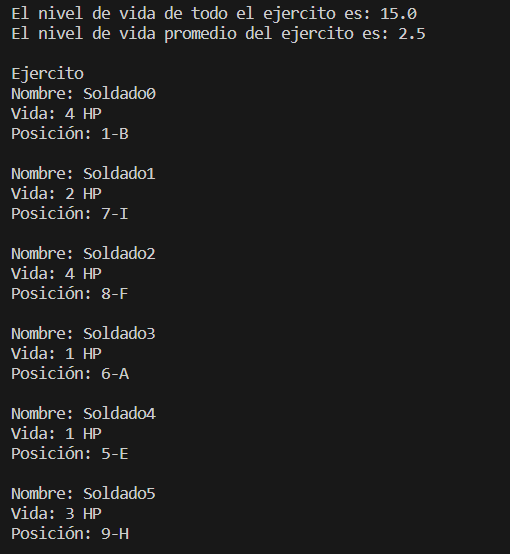
\includegraphics[width=0.4\textwidth,keepaspectratio]{img/captura3.png}
		%\includesvg{img/automata.svg}
		%\label{img:mot2}
		%\caption{Product backlog.}
	\end{figure}
	
	\begin{itemize}	
		\item Ahora seguía algo que ya hemos hecho en laboratorios anteriores, ordenar el ejército por orden de vida, por lo tanto, debíamos implementar algoritmos de ordenamiento necesarios.
		\item Lo primero que hice fue obtener un arreglo unidimensional para poder ordenarlo, en base al tablero que ya tenemos.
	\end{itemize}
	
	\begin{lstlisting}[language=java,caption={Obtener arreglo}, numbers=left][H]
	 public static Soldado[] crearArreglo(Soldado[][] army, int[] filas, int[] columnas) {
        Soldado[] nuevo = new Soldado[filas.length];
        for (int i = 0; i < nuevo.length; i++) {
            nuevo[i] = army[filas[i]][columnas[i]];
        }
        return nuevo;
    }
    
	\end{lstlisting}
	
	\begin{itemize}	
		\item Una vez obtenido el arreglo, solo queda programar los algoritmos de ordenamiento, para esto se pueden reutilizar códigos de clases anteriores.
	\end{itemize}
	
	\begin{lstlisting}[language=java,caption={Algoritmos de ordenamiento}, numbers=left][H]
	 public static void ordenamientoBurbuja(Soldado[] army) {
        for (int i = 0; i < army.length; i++) {
            for (int j = 0; j < army.length - 1; j++) {
                if (army[j].getVida() > army[j + 1].getVida()) {
                    intercambiar(army, j, j + 1);
                }
            }
        }
    }
    public static void intercambiar(Soldado[] flota, int i, int j) {
        Soldado temp;
        temp = flota[i];
        flota[i] = flota[j];
        flota[j] = temp;
    }

    public static void ordenamientoInsercion(Soldado[] army) {
        for (int i = 1; i < army.length; i++) {
            Soldado valor = army[i];
            int j = i;
            for (j = i; 0 < j && army[j - 1].getVida() > valor.getVida(); j--) {
                army[j] = army[j - 1];
            }
            army[j] = valor;
        }
    }
    
	\end{lstlisting}
	
	\begin{lstlisting}[language=java,caption={Metodo main (final)}, numbers=left][H]
	  mostrarEjercito(ejercito, filas, columnas);
        Soldado[] army = crearArreglo(ejercito, filas, columnas);
        System.out.println("Bajo que criterio de ordenamiento le gustaria ordenar el arreglo?");
        System.out.println("1. Burbuja");
        System.out.println("2. Insercion");
        switch (sc.nextInt()) {
            case 1:
                ordenamientoBurbuja(army);
                break;
            case 2:
                ordenamientoInsercion(army);
                break;
            default:
        }
        System.out.println();
        mostrar(army);
    
	\end{lstlisting}
	
	\begin{itemize}	
		\item Aqui solo llamé a todos los métodos desarrollados anteriormente, además de generar como un 'Menú' para que el usuario escoja cómo ordenar el ejército, con diferentes algoritmos de ordenamiento.
		\item En las siguientes capturas, podemos comprobar como funcionan los métodos de ordenamiento.
	\end{itemize}
	
	\begin{figure}[H]
		\centering
		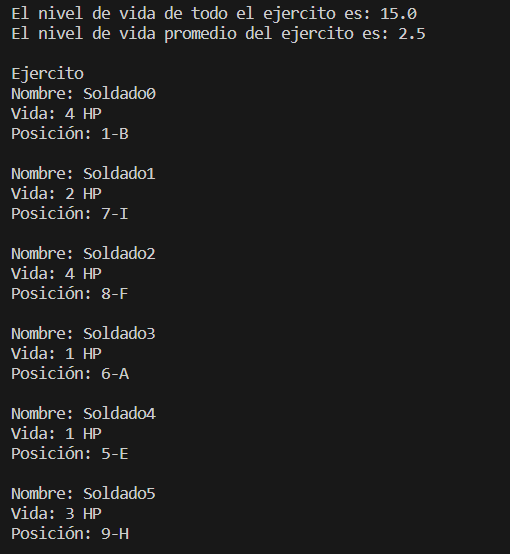
\includegraphics[width=0.8\textwidth,keepaspectratio]{img/captura3.png}
		%\includesvg{img/automata.svg}
		%\label{img:mot2}
		%\caption{Product backlog.}
	\end{figure}
	\begin{itemize}
		\item Ordenando.
	\end{itemize}
	
	\begin{figure}[H]
		\centering
	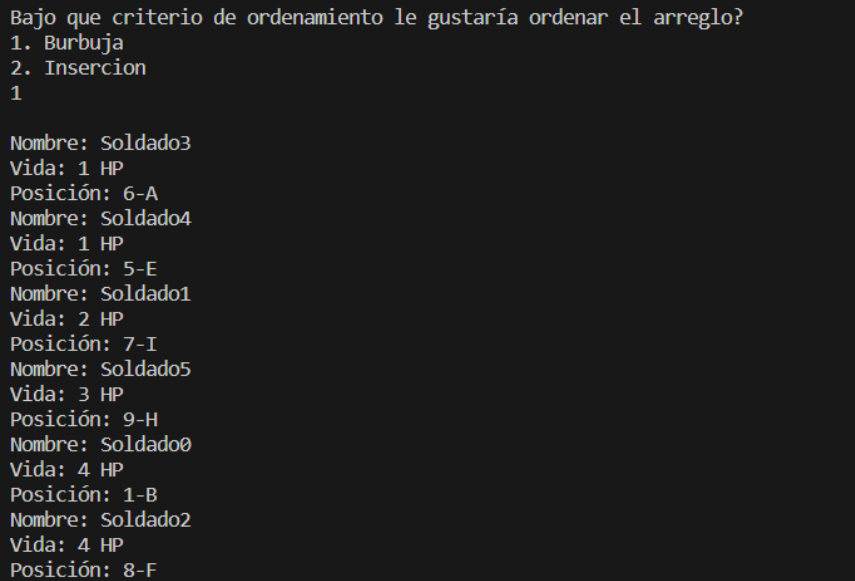
\includegraphics[width=0.8\textwidth,keepaspectratio]{img/captura4.png}
		%\includesvg{img/automata.svg}
		%\label{img:mot2}
		%\caption{Product backlog.}
	\end{figure}
	
	\section{\textcolor{red}{Rúbricas}}
	
	\subsection{\textcolor{red}{Entregable Informe}}
	\begin{table}[H]
		\caption{Tipo de Informe}
		\setlength{\tabcolsep}{0.5em} % for the horizontal padding
		{\renewcommand{\arraystretch}{1.5}% for the vertical padding
		\begin{tabular}{|p{3cm}|p{12cm}|}
			\hline
			\multicolumn{2}{|c|}{\textbf{\textcolor{red}{Informe}}}  \\
			\hline 
			\textbf{\textcolor{red}{Latex}} & \textcolor{blue}{El informe está en formato PDF desde Latex,  con un formato limpio (buena presentación) y facil de leer.}   \\ 
			\hline 
			
			
		\end{tabular}
	}
	\end{table}
	
	\clearpage
	
	\subsection{\textcolor{red}{Rúbrica para el contenido del Informe y demostración}}
	\begin{itemize}			
		\item El alumno debe marcar o dejar en blanco en celdas de la columna \textbf{Checklist} si cumplio con el ítem correspondiente.
		\item Si un alumno supera la fecha de entrega,  su calificación será sobre la nota mínima aprobada, siempre y cuando cumpla con todos lo items.
		\item El alumno debe autocalificarse en la columna \textbf{Estudiante} de acuerdo a la siguiente tabla:
	
		\begin{table}[ht]
			\caption{Niveles de desempeño}
			\begin{center}
			\begin{tabular}{ccccc}
    			\hline
    			 & \multicolumn{4}{c}{Nivel}\\
    			\cline{1-5}
    			\textbf{Puntos} & Insatisfactorio 25\%& En Proceso 50\% & Satisfactorio 75\% & Sobresaliente 100\%\\
    			\textbf{2.0}&0.5&1.0&1.5&2.0\\
    			\textbf{4.0}&1.0&2.0&3.0&4.0\\
    		\hline
			\end{tabular}
		\end{center}
	\end{table}	
	
	\end{itemize}
	
	\begin{table}[H]
		\caption{Rúbrica para contenido del Informe y demostración}
		\setlength{\tabcolsep}{0.5em} % for the horizontal padding
		{\renewcommand{\arraystretch}{1.5}% for the vertical padding
		%\begin{center}
		\begin{tabular}{|p{2.7cm}|p{7cm}|x{1.3cm}|p{1.2cm}|p{1.5cm}|p{1.1cm}|}
			\hline
    		\multicolumn{2}{|c|}{Contenido y demostración} & Puntos & Checklist & Estudiante & Profesor\\
			\hline
			\textbf{1. GitHub} & Hay enlace URL activo del directorio para el  laboratorio hacia su repositorio GitHub con código fuente terminado y fácil de revisar. &2 &X &2 & \\ 
			\hline
			\textbf{2. Commits} &  Hay capturas de pantalla de los commits más importantes con sus explicaciones detalladas. (El profesor puede preguntar para refrendar calificación). &4 &X &2 & \\ 
			\hline 
			\textbf{3. Código fuente} &  Hay porciones de código fuente importantes con numeración y explicaciones detalladas de sus funciones. &2 &X &2 & \\ 
			\hline 
			\textbf{4. Ejecución} & Se incluyen ejecuciones/pruebas del código fuente  explicadas gradualmente. &2 &X &2 & \\ 
			\hline			
			\textbf{5. Pregunta} & Se responde con completitud a la pregunta formulada en la tarea.  (El profesor puede preguntar para refrendar calificación).  &2 &X &2 & \\ 
			\hline	
			\textbf{6. Fechas} & Las fechas de modificación del código fuente estan dentro de los plazos de fecha de entrega establecidos. &2 &X &2 & \\ 
			\hline 
			\textbf{7. Ortografía} & El documento no muestra errores ortográficos. &2 &X &2 & \\ 
			\hline 
			\textbf{8. Madurez} & El Informe muestra de manera general una evolución de la madurez del código fuente,  explicaciones puntuales pero precisas y un acabado impecable.   (El profesor puede preguntar para refrendar calificación).  &4 &X &4 & \\ 
			\hline
			\multicolumn{2}{|c|}{\textbf{Total}} &20 & &18 & \\ 
			\hline
		\end{tabular}
		%\end{center}
		%\label{tab:multicol}
		}
	\end{table}
	
\clearpage

\section{Referencias}
	\begin{itemize}
		\item Fundamentos de la programación 2 - Tópicos de la programación Orientada a Objetos (Marco Aedo)
	\end{itemize}
	
%\clearpage
%\bibliographystyle{apalike}
%\bibliographystyle{IEEEtranN}
%\bibliography{bibliography}
			
\end{document}
